\documentclass[a4paper,utf8]{article}
\usepackage{exemple}
\usepackage[normalem]{ulem}
\usepackage{amsfonts}
\usepackage{graphicx}
\usepackage{MnSymbol,wasysym}
\usepackage{hyperref}
\usepackage[french]{babel}
\usepackage{graphicx}

\formation{L3MI}
\date{}
\matiere{Conception Orient�e Objet}
\titre{Projet : Tetris Attck }

\newcommand\code[1]{\textsf{#1}}
\newcommand\srdjan[1]{{\color{red} #1}}

\begin{document}

\entete

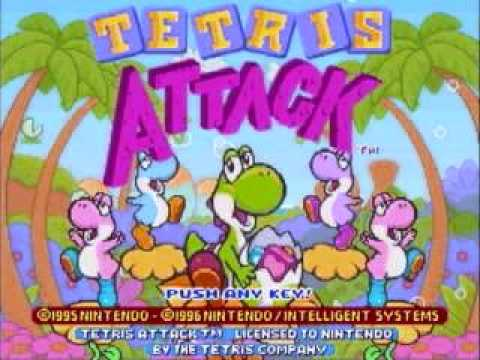
\includegraphics{img1.jpg}

\section{Description du Projet}
Tetris Attack est un puzzle-game `a 2 joueurs sorti en 1995 sur Super Nintendo. Ce jeu est une variante du bien connu Tetris a 2 joueurs. Dans cette version, l?objectif est d?assembler des blocs entre eux afin de les faire dispara??tre avant que l?ensemble des blocs n?atteignent le haut de l? ?ecran. Toutefois, ici, 2 joueurs s?affrontent en parall`ele et peuvent `a l?aide de diff ?erentes combinaisons envoyer de nouveaux blocs de briques `a leur adversaire afin de pr ?ecipiter sa perte. Ce jeu couple `a la fois, la simplicit ?e de Tetris `a la dynamicit ?e n ?ecessaire d?un bon Versus.

\section{L'Organisation }

\subsection{Gantt}
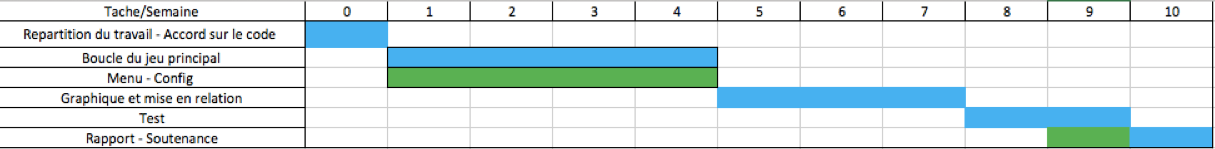
\includegraphics[scale=0.9]{gant.png}
\subsection{L'Equipe}

\begin{itemize}
\item vincent : jeu principal , graphique , ia 
\item loick : jeu principal , graphique , ia 
\item mohammed: menu , diff�rent ecran pour config , graphique
\item kevin: menu , diff�rent ecran pour config , graphique
\end{itemize}

\section{Le rendu du Projet }

\subsection{Les ecrans de Jeux}

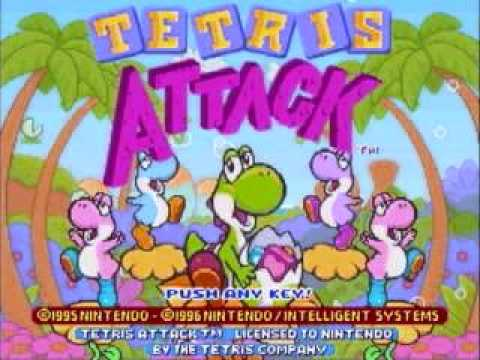
\includegraphics[scale=0.4]{img1.jpg}

\subsection{Le Menu}

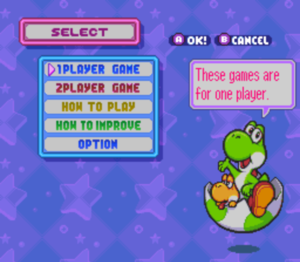
\includegraphics[scale=0.6]{img2.png}

\subsection{L'ecran de jeu}

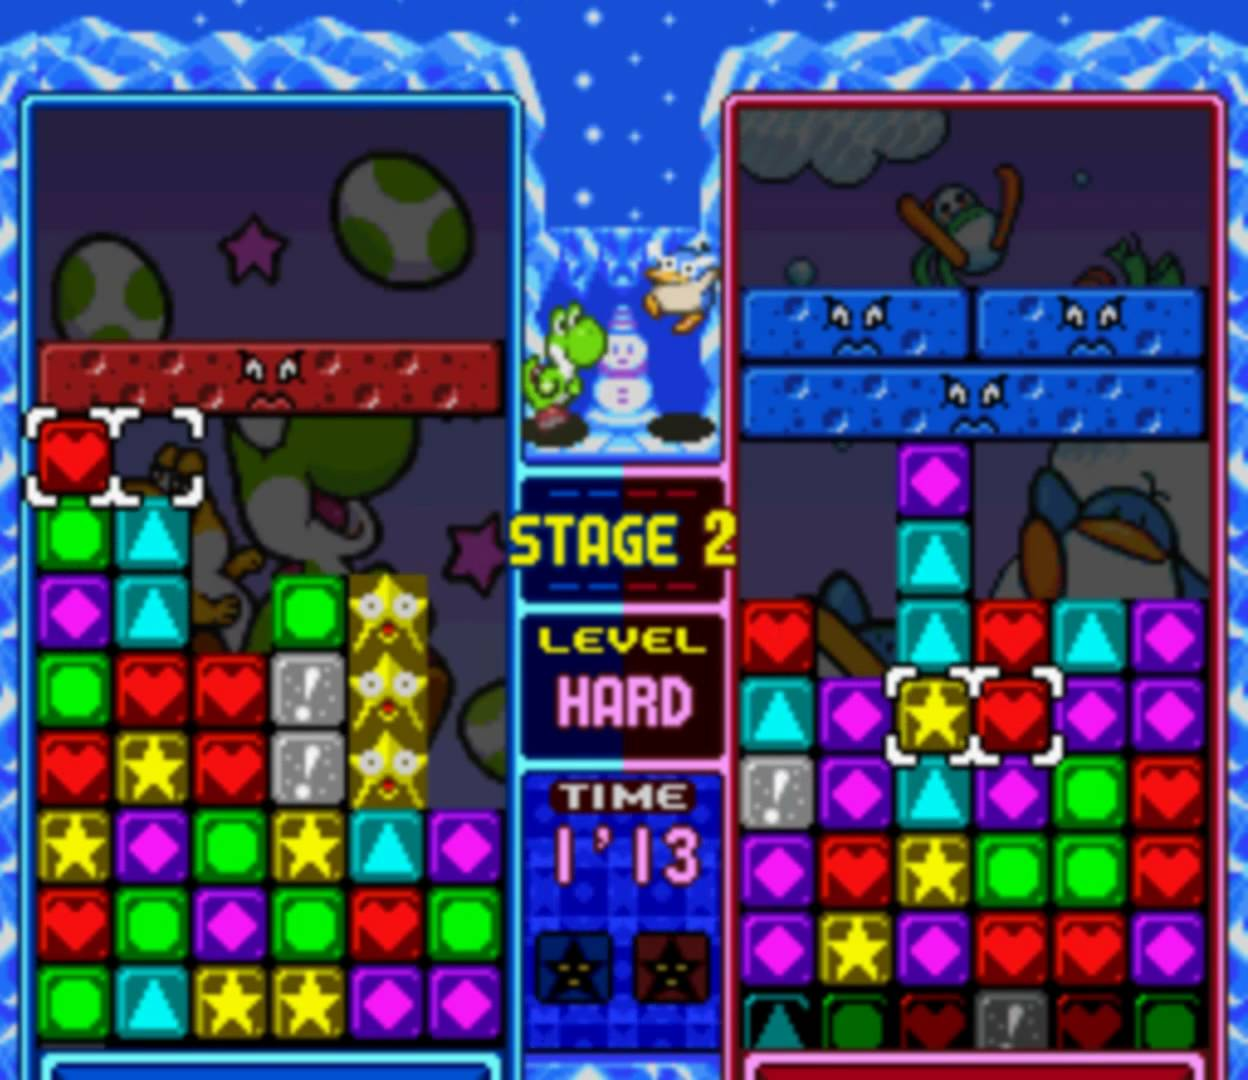
\includegraphics[scale=0.15]{img3.jpg}
\ldots

\end{document}
